\hypertarget{digital-signal-processing-dsp---session-4}{%
\section{Digital Signal Processing (DSP) - Session
4}\label{digital-signal-processing-dsp---session-4}}

\begin{center}\rule{0.5\linewidth}{0.5pt}\end{center}

\hypertarget{the-z-transform-and-its-application-to-the-analysis-of-lti-systems}{%
\subsection{The Z-Transform and Its Application to the Analysis of LTI
Systems}\label{the-z-transform-and-its-application-to-the-analysis-of-lti-systems}}

\begin{quote}
\textbf{\emph{Example 1.2}}

Determine the z-transform of the signal

\[x(n) = (\frac{1}{2})^nu(n)\]

\emph{Solution}

\begin{enumerate}
\def\labelenumi{\arabic{enumi}.}
\item
  \textbf{Apply the Z-Transform Definition}: The z-transform is defined
  by the power series: \[X(z) = \sum_{n=-\infty}^{\infty} x(n)z^{-n}\]
\item
  \textbf{Substitute the Signal}: Since the unit step signal
  \textbf{\(u(n)\)} is \(1\) for \(n \ge 0\) and \(0\) for \(n < 0\),
  change the summation limits:
  \[X(z) = \sum_{n=0}^{\infty} \left(\frac{1}{2}\right)^n z^{-n}\]
\item
  \textbf{Rewrite as a Single Power}: Combine the terms into a geometric
  series form:
  \[X(z) = \sum_{n=0}^{\infty} \left(\frac{1}{2} z^{-1}\right)^n\]
\item
  \textbf{Use Geometric Series Summation}: Recall the sum formula for an
  infinite geometric series: \(\sum_{n=0}^{\infty} A^n = \frac{1}{1-A}\)
  if \(|A| < 1\). Here, \(A = \frac{1}{2} z^{-1}\).
\item
  \textbf{Determine the Closed-Form Expression}: Substitute \(A\) into
  the formula: \textbf{\[X(z) = \frac{1}{1 - \frac{1}{2} z^{-1}}\]}
\item
  \textbf{Find the Region of Convergence (ROC)}: The series converges
  only if \(|\frac{1}{2} z^{-1}| < 1\). Solving for \(z\):
  \(\frac{1}{2} |z|^{-1} < 1 \implies \frac{1}{2|z|} < 1 \implies\)
  \textbf{\(|z| > \frac{1}{2}\)}.
\end{enumerate}
\end{quote}

\begin{quote}
\textbf{\emph{Example 1.3}}

Determine the \textbf{z-transform} of the exponential signal:

\[
x(n) = \alpha^n u(n) =
\begin{cases}
\alpha^n, & n \ge 0 \\
0, & n < 0 
\end{cases}
\]

\emph{Solution}

\begin{enumerate}
\def\labelenumi{\arabic{enumi}.}
\tightlist
\item
  \textbf{Use the Z-Transform Definition}: Apply the standard power
  series formula: \[X(z) = \sum_{n=-\infty}^{\infty} x(n)z^{-n}\]
\item
  \textbf{Substitute the Signal}: Since the unit step \(u(n)\) is zero
  for \(n < 0\), adjust the summation limits:
  \[X(z) = \sum_{n=0}^{\infty} \alpha^n z^{-n}\]
\item
  \textbf{Rewrite as a Geometric Series}: Combine the terms into a
  single power of \(n\):
  \[X(z) = \sum_{n=0}^{\infty} (\alpha z^{-1})^n\]
\item
  \textbf{Apply Geometric Series Summation}: Use the sum formula
  \(\sum_{n=0}^{\infty} A^n = \frac{1}{1-A}\), which is valid for
  \(|A| < 1\).
\item
  \textbf{Form the Closed-Form Expression}: Substitute
  \(A = \alpha z^{-1}\) into the sum formula:
  \textbf{\[X(z) = \frac{1}{1 - \alpha z^{-1}}\]}
\item
  \textbf{Determine the Region of Convergence (ROC)}: The series
  converges only if \(|\alpha z^{-1}| < 1\). Solving for \(z\) yields:
  \textbf{\(|z| > |\alpha|\)}
\end{enumerate}
\end{quote}

\begin{quote}
\textbf{\emph{Example 1.4}}

Determine the \textbf{z-transform} of the anticausal signal: \[
x(n) = -\alpha^n u(-n-1) =
\begin{cases} 0, & n \ge 0 \\
-\alpha^n, & n \le -1 
\end{cases}
\]

\emph{Solution}

\begin{enumerate}
\def\labelenumi{\arabic{enumi}.}
\tightlist
\item
  \textbf{Use the Z-Transform Definition}: Apply the standard power
  series formula: \(X(z) = \sum_{n=-\infty}^{\infty} x(n)z^{-n}\).
\item
  \textbf{Substitute the Signal}: Adjust the limits for the anticausal
  signal: \[X(z) = \sum_{n=-\infty}^{-1} (-\alpha^n) z^{-n}\]
\item
  \textbf{Change Variable for Summation}: Let \(l = -n\). The sum
  becomes: \[X(z) = -\sum_{l=1}^{\infty} (\alpha^{-1} z)^l\]
\item
  \textbf{Apply Geometric Series Summation}: Use the formula
  \(A + A^2 + A^3 + \dots = \frac{A}{1-A}\) for \(|A| < 1\).
\item
  \textbf{Form the Closed-Form Expression}: Substitute
  \(A = \alpha^{-1} z\) into the formula and simplify:
  \[X(z) = -\frac{\alpha^{-1} z}{1 - \alpha^{-1} z} = \mathbf{\frac{1}{1 - \alpha z^{-1}}}\]
\item
  \textbf{Determine the Region of Convergence (ROC)}: The series
  converges only if \(|\alpha^{-1} z| < 1\). Solving for \(z\) yields
  the interior of a circle: \textbf{\(|z| < |\alpha|\)}
\end{enumerate}
\end{quote}

\textbf{Note:} Examples 1.3 and 1.4 highlight that a closed-form
expression does not uniquely specify a signal; both the expression and
the \textbf{ROC} are required for uniqueness.

\begin{quote}
\textbf{\emph{Example 1.5}}

Determine the \textbf{z-transform} of the two-sided signal:
\[x(n) = \alpha^n u(n) + b^n u(-n-1)\]

\emph{Solution}

\begin{enumerate}
\def\labelenumi{\arabic{enumi}.}
\tightlist
\item
  \textbf{Use the Z-Transform Definition}: Apply the standard power
  series formula: \(X(z) = \sum_{n=-\infty}^{\infty} x(n)z^{-n}\).
\item
  \textbf{Substitute the Signal Components}: Split the summation into
  two parts corresponding to the causal and anticausal terms:
  \[X(z) = \sum_{n=0}^{\infty} \alpha^n z^{-n} + \sum_{n=-\infty}^{-1} b^n z^{-n}\]
\item
  \textbf{Rewrite as Geometric Series}:

  \begin{itemize}
  \tightlist
  \item
    \textbf{Part 1}: \(\sum_{n=0}^{\infty} (\alpha z^{-1})^n\).
  \item
    \textbf{Part 2}: Let \(l = -n\). The sum becomes
    \(\sum_{l=1}^{\infty} (b^{-1} z)^l\).
  \end{itemize}
\item
  \textbf{Determine Convergence Conditions}:

  \begin{itemize}
  \tightlist
  \item
    The first series converges if \(|\alpha z^{-1}| < 1 \implies\)
    \textbf{\(|z| > |\alpha|\)}.
  \item
    The second series converges if \(|b^{-1} z| < 1 \implies\)
    \textbf{\(|z| < |b|\)}.
  \end{itemize}
\item
  \textbf{Analyze the Region of Convergence (ROC)}:

  \begin{itemize}
  \tightlist
  \item
    If \textbf{\(|b| < |\alpha|\)}, there is no common region of
    convergence; thus, \textbf{\(X(z)\) does not exist}.
  \item
    If \textbf{\(|\alpha| < |b|\)}, the common region is the ring
    between the two circles: \textbf{\(|\alpha| < |z| < |b|\)}.
  \end{itemize}
\item
  \textbf{Form the Closed-Form Expression}: If the ROC exists
  (\(|\alpha| < |b|\)), combine the results of the two geometric series:
  \[X(z) = \frac{1}{1 - \alpha z^{-1}} - \frac{1}{1 - b z^{-1}}\] Which
  simplifies to:
  \textbf{\[X(z) = \frac{(b - \alpha) z^{-1}}{(1 - \alpha z^{-1})(1 - b z^{-1})}\]}
\end{enumerate}
\end{quote}

\hypertarget{the-inverse-z-transform}{%
\subsubsection{The Inverse z-Transform}\label{the-inverse-z-transform}}

\begin{itemize}
\tightlist
\item
  \textbf{Definition}: The procedure used to recover the time-domain
  signal \(x(n)\) from its complex-plane representation \(X(z)\).
\item
  \textbf{Mathematical Basis}: Derived using the \textbf{Cauchy integral
  theorem}.
\item
  \textbf{Inversion Formula}:
  \[x(n) = \frac{1}{2\pi j} \oint_C X(z)z^{n-1} dz\] where \(C\) is a
  counterclockwise closed contour within the \textbf{Region of
  Convergence (ROC)} that encloses the origin.
\item
  \textbf{Practical Methods of Inversion}:

  \begin{enumerate}
  \def\labelenumi{\arabic{enumi}.}
  \tightlist
  \item
    \textbf{Contour Integration}: Direct evaluation of the integral by
    summing the residues of \(X(z)z^{n-1}\) at the poles inside the
    contour \(C\).
  \item
    \textbf{Power Series Expansion}: Expanding \(X(z)\) into a series
    (often via \textbf{long division}); the coefficients of the
    resulting \(z^{-n}\) terms represent the values of \(x(n)\).
  \item
    \textbf{Partial-Fraction Expansion}: Decomposing a rational
    \(z\)-transform into simpler fractions that can be inverted using a
    \textbf{table lookup} and the linearity property.
  \end{enumerate}
\end{itemize}

\hypertarget{properties-of-the-z-transform}{%
\subsubsection{Properties of the
z-Transform}\label{properties-of-the-z-transform}}

\begin{itemize}
\tightlist
\item
  \textbf{Linearity}: The z-transform of a linear combination of signals
  equals the same linear combination of their individual transforms:
  \[a_1x_1(n) + a_2x_2(n) \leftrightarrow a_1X_1(z) + a_2X_2(z)\]
\item
  \textbf{Time shifting}: Shifting a signal by \(k\) samples corresponds
  to multiplication by \(z^{-k}\):
  \[x(n - k) \leftrightarrow z^{-k}X(z)\] The ROC remains unchanged
  except possibly at \(z=0\) or \(z=\infty\).
\item
  \textbf{Scaling in the z-domain}: Multiplying a signal by an
  exponential sequence \(a^n\) scales the complex variable \(z\):
  \[a^nx(n) \leftrightarrow X(a^{-1}z)\] The ROC is scaled by \(|a|\).
\item
  \textbf{Time reversal}: Reflecting a signal in the time domain
  corresponds to inverting the \(z\) variable:
  \[x(-n) \leftrightarrow X(z^{-1})\] The ROC is inverted
  (\(1/r_2 < |z| < 1/r_1\)).
\item
  \textbf{Differentiation in the z-domain}: Multiplying a signal by
  \(n\) corresponds to differentiation in the z-domain:
  \[nx(n) \leftrightarrow -z \frac{dX(z)}{dz}\] The ROC remains the
  same.
\item
  \textbf{Convolution of two sequences}: Convolution in the time domain
  is equivalent to multiplication in the z-domain:
  \[x_1(n) * x_2(n) \leftrightarrow X_1(z)X_2(z)\] The ROC is at least
  the intersection of individual ROCs.
\item
  \textbf{Correlation of two sequences}: The transform of the
  crosscorrelation of two signals is:
  \[r_{x_1x_2}(l) \leftrightarrow R_{x_1x_2}(z) = X_1(z)X_2(z^{-1})\]
\item
  \textbf{Multiplication of two sequences}: Multiplication in the time
  domain corresponds to a complex convolution integral in the z-domain:
  \[x_1(n)x_2(n) \leftrightarrow \frac{1}{2\pi j} \oint_C X_1(v)X_2(z/v)v^{-1}dv\]
\item
  \textbf{Parseval's relation}: Relates the energy of signals in the
  time domain to an integral in the z-domain:
  \[\sum_{n=-\infty}^{\infty} x_1(n)x_2^*(n) = \frac{1}{2\pi j} \oint_C X_1(v)X_2^*(1/v^*)v^{-1}dv\]
\item
  \textbf{The Initial Value Theorem}: For a causal signal (\(x(n) = 0\)
  for \(n < 0\)), the initial value can be found by:
  \[x(0) = \lim_{z \to \infty} X(z)\]
\end{itemize}

\begin{quote}
\textbf{\emph{Example 2.1}}

Determine the \textbf{z-transform} and the \textbf{Region of Convergence
(ROC)} of the signal: \[x(n) = [3(2^n) - 4(3^n)]u(n)\]

\emph{Solution}

\begin{enumerate}
\def\labelenumi{\arabic{enumi}.}
\tightlist
\item
  \textbf{Define Signal Components}: Let \(x_1(n) = 2^n u(n)\) and
  \(x_2(n) = 3^n u(n)\).
\item
  \textbf{Apply Linearity}: The signal is a linear combination:
  \(x(n) = 3x_1(n) - 4x_2(n)\). The property states:
  \(X(z) = 3X_1(z) - 4X_2(z)\).
\item
  \textbf{Find Individual Transforms and ROCs}:

  \begin{itemize}
  \tightlist
  \item
    \textbf{For \(x_1(n)\)}: Using the pair
    \(\alpha^n u(n) \leftrightarrow \frac{1}{1-\alpha z^{-1}}\), we get
    \(X_1(z) = \frac{1}{1-2z^{-1}}\) with \textbf{ROC: \(|z| > 2\)}.
  \item
    \textbf{For \(x_2(n)\)}: Similarly, \(X_2(z) = \frac{1}{1-3z^{-1}}\)
    with \textbf{ROC: \(|z| > 3\)}.
  \end{itemize}
\item
  \textbf{Form the Combined Expression}: Substitute these into the
  linear equation:
  \textbf{\[X(z) = \frac{3}{1-2z^{-1}} - \frac{4}{1-3z^{-1}}\]}
\item
  \textbf{Determine Overall ROC}: The overall ROC is the
  \textbf{intersection} of the individual ROCs (\(|z| > 2\) and
  \(|z| > 3\)). \textbf{ROC: \(|z| > 3\)}
\end{enumerate}
\end{quote}

\begin{quote}
\textbf{\emph{Proof of the time shifting property}}

Let \(y(n) = x(n - k)\) be the shifted signal. We determine its
z-transform \(Y(z)\) using the definition:
\[Y(z) = \sum_{n=-\infty}^{\infty} y(n)z^{-n} = \sum_{n=-\infty}^{\infty} x(n - k)z^{-n}\]

To solve this, we make a \textbf{change of variable}. Let
\textbf{\(m = n - k\)}, which implies that \textbf{\(n = m + k\)}. As
\(n\) ranges from \(-\infty\) to \(\infty\), \(m\) also ranges from
\(-\infty\) to \(\infty\). Substituting these into the summation:
\[Y(z) = \sum_{m=-\infty}^{\infty} x(m)z^{-(m+k)}\]

Using the properties of exponents (\(z^{-(m+k)} = z^{-m}z^{-k}\)), we
can rewrite the expression:
\[Y(z) = \sum_{m=-\infty}^{\infty} x(m)z^{-m}z^{-k}\]

Since \(z^{-k}\) does not depend on the summation index \(m\), we can
factor it out of the sum:
\[Y(z) = z^{-k} \sum_{m=-\infty}^{\infty} x(m)z^{-m}\]

We recognize that the remaining summation is the definition of the
z-transform \(X(z)\). Therefore: \textbf{\[Y(z) = z^{-k}X(z)\]}
\end{quote}

\begin{quote}
\textbf{\emph{Proof of the convolution of two sequences property}}

The convolution of \(x_1(n)\) and \(x_2(n)\) is defined as:
\[x(n) = x_1(n) * x_2(n) = \sum_{k=-\infty}^{\infty} x_1(k)x_2(n-k)\]

By the definition of the direct z-transform, we have:
\[X(z) = \sum_{n=-\infty}^{\infty} x(n)z^{-n} = \sum_{n=-\infty}^{\infty} \left[ \sum_{k=-\infty}^{\infty} x_1(k)x_2(n-k) \right] z^{-n}\]

Rearrange the terms to group those dependent on \(n\):
\[X(z) = \sum_{k=-\infty}^{\infty} x_1(k) \left[ \sum_{n=-\infty}^{\infty} x_2(n-k)z^{-n} \right]\]

The inner summation is the z-transform of the shifted sequence
\(x_2(n - k)\). According to the \textbf{time-shifting property},
\[x_2(n - k) \leftrightarrow z^{-k}X_2(z)\]

Substituting this into the equation:
\[X(z) = \sum_{k=-\infty}^{\infty} x_1(k) \left[ z^{-k}X_2(z) \right]\]

Since \(X_2(z)\) does not depend on the summation index \(k\), it can be
moved outside the sum:
\[X(z) = X_2(z) \sum_{k=-\infty}^{\infty} x_1(k)z^{-k}\] The remaining
sum is the definition of \(X_1(z)\). Thus:
\textbf{\[X(z) = X_1(z)X_2(z)\]}
\end{quote}

\hypertarget{poles-and-zeros}{%
\subsubsection{Poles and Zeros}\label{poles-and-zeros}}

\begin{itemize}
\item
  \textbf{Definitions}:

  \begin{itemize}
  \tightlist
  \item
    \textbf{Zeros}: The values of \(z\) for which \(H(z) = 0\).
  \item
    \textbf{Poles}: The values of \(z\) for which \(H(z) = \infty\).
  \end{itemize}
\item
  \textbf{Rational System Function (Standard Form)}: Assuming
  \(a_0 = 1\) for a linear constant-coefficient difference equation:
  \[H(z) = \frac{Y(z)}{X(z)} = \frac{\sum_{k=0}^{M} b_k z^{-k}}{\sum_{k=0}^{N} a_k z^{-k}}\]
\item
  \textbf{Factored (Pole-Zero) Form}: Factoring the polynomials reveals
  the specific locations of the zeros (\(z_k\)) and poles (\(p_k\)):
  \[H(z) = G z^{N-M} \frac{(z - z_1)(z - z_2) \dots (z - z_M)}{(z - p_1)(z - p_2) \dots (z - p_N)}\]

  \begin{itemize}
  \tightlist
  \item
    \textbf{Gain Factor (\(G\))}: Defined as \(b_0/a_0\).
  \item
    \textbf{Trivial Singularities}: The term \(z^{N-M}\) represents
    additional zeros (if \(N > M\)) or poles (if \(N < M\)) located at
    the \textbf{origin (\(z = 0\))}.
  \end{itemize}
\item
  \textbf{Graphical Representation (Pole-Zero Plot)}:

  \begin{itemize}
  \tightlist
  \item
    \textbf{Poles} are indicated by crosses (\(\times\)).
  \item
    \textbf{Zeros} are indicated by circles (\(\circ\)).
  \item
    \textbf{Multiplicity}: If a pole or zero occurs more than once at
    the same location, the order is noted next to the mark.
  \end{itemize}
\item
  \textbf{Relationship to ROC}:

  \begin{itemize}
  \tightlist
  \item
    By definition, the \textbf{Region of Convergence (ROC)} of a
    z-transform cannot contain any poles.
  \item
    The transform does not converge at a pole because the value becomes
    infinite.
  \end{itemize}
\end{itemize}

\begin{quote}
\textbf{\emph{Example}}

Determine \(H(z)\) for this system:

\[y(n) = x(n) - \frac{1}{2}x(n-2) - y(n-1)\]

\emph{Solution}

\textbf{1. Rearrange the Difference Equation}

First, group all the terms involving the output \(y(n)\) on one side and
the terms involving the input \(x(n)\) on the other:
\[y(n) + y(n-1) = x(n) - \frac{1}{2}x(n-2)\]

\textbf{2. Apply the Z-Transform}

Next, take the z-transform of both sides of the equation. According to
the \textbf{time-shifting property}, a delay of \(k\) samples in the
time domain corresponds to multiplying by \(z^{-k}\) in the z-domain
(\(x(n-k) \leftrightarrow z^{-k}X(z)\)):
\[Y(z) + z^{-1}Y(z) = X(z) - \frac{1}{2}z^{-2}X(z)\]

\textbf{3. Factor and Solve for \(H(z)\)}

Factor out \(Y(z)\) and \(X(z)\) from their respective sides:
\[Y(z)(1 + z^{-1}) = X(z)\left(1 - \frac{1}{2}z^{-2}\right)\]

The system function \textbf{\(H(z)\)} is defined as the ratio of the
output transform to the input transform:
\[H(z) = \frac{Y(z)}{X(z)} = \frac{1 - \frac{1}{2}z^{-2}}{1 + z^{-1}}\]
\end{quote}

\begin{quote}
\textbf{\emph{Example 3.1}}

Determine the pole-zero plot for the signal

\[
x(n) = a^n u(n), \quad a > 0
\]

\emph{Solution}

\begin{enumerate}
\def\labelenumi{\arabic{enumi}.}
\tightlist
\item
  \textbf{Compute the \(z\)-transform}: Using the direct \(z\)-transform
  formula,
  \[X(z) = \sum_{n=0}^{\infty} a^n z^{-n} = \sum_{n=0}^{\infty} (az^{-1})^n\]
  This geometric series converges when \(|az^{-1}| < 1\), resulting in:
  \[X(z) = \frac{1}{1 - az^{-1}}\]
\item
  \textbf{Express as a rational function}: Convert the expression to use
  positive powers of \(z\) by multiplying the numerator and denominator
  by \(z\): \[X(z) = \frac{z}{z - a}\]
\item
  \textbf{Identify zeros and poles}:

  \begin{itemize}
  \tightlist
  \item
    \textbf{Zeros}: The values of \(z\) where the numerator is zero.
    Here, \(X(z) = 0\) at \textbf{\(z_1 = 0\)}.
  \item
    \textbf{Poles}: The values of \(z\) where the denominator is zero
    (making \(X(z)\) infinite). here, \(X(z) = \infty\) at
    \textbf{\(p_1 = a\)}
  \end{itemize}
\item
  \textbf{Determine the Region of Convergence (ROC)}: For a causal
  signal, the ROC is the exterior of a circle of radius equal to the
  magnitude of the largest pole. Thus, the \textbf{ROC is \(|z| > a\)}
\end{enumerate}
\end{quote}

\begin{quote}
\textbf{\emph{Example 3.2}}

Determine the pole-zero plot for the signal:

\[
x(n) =
\begin{cases}
a^n, & 0 \le n \le M-1 \\
0, & \text{elsewhere}
\end{cases}
\]

where \(a > 0\).

\emph{Solution}

\begin{enumerate}
\def\labelenumi{\arabic{enumi}.}
\tightlist
\item
  \textbf{Apply the Z-transform definition:}
  \[X(z) = \sum_{n=0}^{M-1} a^n z^{-n} = \sum_{n=0}^{M-1} (az^{-1})^n\]
\item
  \textbf{Use the finite geometric series formula:}
  \[X(z) = \frac{1 - (az^{-1})^M}{1 - az^{-1}}\]
\item
  \textbf{Rearrange into positive powers of \(z\):} Multiply the
  numerator and denominator by \(z^M\):
  \[X(z) = \frac{z^M - a^M}{z^{M-1}(z - a)}\]
\item
  \textbf{Find the zeros:} Zeros occur where the numerator is zero:
  \(z^M - a^M = 0\). The \(M\) roots are:
  \textbf{\(z_k = a e^{j 2\pi k / M}\)} for \(k = 0, 1, \dots, M-1\).
\item
  \textbf{Find the poles:} The denominator indicates \(M-1\) poles at
  \textbf{\(z = 0\)} (the origin) and one pole at \textbf{\(z = a\)}.
\item
  \textbf{Identify pole-zero cancellation:} For \(k = 0\), the zero is
  \(z_0 = a e^{j0} = a\). This \textbf{zero at \(z = a\) cancels the
  pole at \(z = a\)}.
\item
  \textbf{Final Result:}

  \begin{itemize}
  \tightlist
  \item
    \textbf{Zeros:} \(M-1\) zeros located on a circle of radius \(a\) at
    \(z_k = a e^{j 2\pi k / M}\) for \(k = 1, 2, \dots, M-1\).
  \item
    \textbf{Poles:} \(M-1\) poles located at the origin (\(z = 0\)).
  \end{itemize}
\end{enumerate}
\end{quote}

\hypertarget{analysis-of-linear-time-invariant-systems-in-the-z-domain}{%
\subsubsection{Analysis of Linear Time-Invariant Systems in the
z-Domain}\label{analysis-of-linear-time-invariant-systems-in-the-z-domain}}

\begin{itemize}
\item
  \textbf{Response of Systems with Rational System Functions}

  \begin{itemize}
  \tightlist
  \item
    Linear time-invariant (LTI) systems described by
    constant-coefficient difference equations have \textbf{rational
    system functions} of the form \[H(z) = \frac{B(z)}{A(z)}\]
  \item
    For a relaxed system, the output \(z\)-transform is the product of
    the system function and the input \(z\)-transform:
    \[Y(z) = H(z)X(z)\]
  \item
    The total response \(y(n)\) can be subdivided into two parts:

    \begin{itemize}
    \tightlist
    \item
      \textbf{Natural Response}: Determined by the poles \({p_k}\) of
      the system.
    \item
      \textbf{Forced Response}: Determined by the poles \({q_k}\) of the
      input signal.
    \end{itemize}
  \item
    The system's influence on the forced response and the input signal's
    influence on the natural response are exerted through scale factors
    (residues) determined during partial-fraction expansion.
  \end{itemize}
\item
  \textbf{Transient and Steady-State Responses}

  \begin{itemize}
  \tightlist
  \item
    \textbf{Transient Response}: In a stable system, all poles lie
    inside the unit circle (\(|p_k| < 1\)), causing the natural response
    to decay to zero as \(n \to \infty\).
  \item
    \textbf{Steady-State Response}: If the input signal is a sinusoid
    (poles on the unit circle), the forced response persists for all
    \(n \ge 0\).
  \item
    A system only sustains a steady-state output if the input signal
    itself persists (e.g., a sinusoid applied at \(n=0\) that does not
    decay).
  \end{itemize}
\item
  \textbf{Causality and Stability}

  \begin{itemize}
  \tightlist
  \item
    \textbf{Causality}: An LTI system is causal if and only if the
    region of convergence (ROC) of its system function is the
    \textbf{exterior of a circle}, including \(z = \infty\).
  \item
    \textbf{Stability}: An LTI system is BIBO stable if and only if the
    \textbf{unit circle (\(|z| = 1\)) is contained within the ROC} of
    the system function \(H(z)\).
  \item
    \textbf{Combined Requirement}: A causal LTI system is BIBO stable if
    and only if \textbf{all poles of \(H(z)\) lie strictly inside the
    unit circle}.
  \end{itemize}
\item
  \textbf{Pole-Zero Cancellations}

  \begin{itemize}
  \tightlist
  \item
    Occurs when a pole and zero are at the identical location, causing
    the term associated with that pole to vanish from the inverse
    \(z\)-transform.
  \item
    This can be used to \textbf{reduce the order of a system} or to
    suppress specific modes of an input signal.
  \item
    In practice, one should not attempt to stabilize an unstable system
    by placing a zero over an unstable pole because any numerical
    imprecision will prevent exact cancellation, likely leaving the
    system unstable.
  \end{itemize}
\item
  \textbf{Multiple-Order Poles and Stability}

  \begin{itemize}
  \tightlist
  \item
    If a system pole lies on the unit circle, the system is generally
    \textbf{unstable} because a matching pole in a bounded input (like a
    unit step) will create a multiple-order pole on the unit circle,
    resulting in an unbounded output (e.g., a ramp signal).
  \item
    Stable systems must have poles strictly inside the unit circle;
    matching input poles will still result in terms like \(n^{b} p_k^n\)
    in the output, but these will decay as \(n \to \infty\) because the
    exponential factor \(p_k^n\) dominates the polynomial \(n^b\) when
    \(|p_k| < 1\).
  \item
    Systems with distinct poles on the unit circle (like digital
    oscillators) are often called \textbf{marginally stable}.
  \end{itemize}
\item
  \textbf{Stability of Second-Order Systems}

  \begin{itemize}
  \tightlist
  \item
    A causal two-pole system with
    \[H(z) = \frac{b_0}{1 + a_1 z^{-1} + a_2 z^{-2}}\] is stable if its
    poles lie inside the unit circle.
  \item
    This condition is satisfied if the coefficients \((a_1, a_2)\) fall
    within the \textbf{stability triangle} defined by:

    \begin{itemize}
    \tightlist
    \item
      \(|a_2| < 1\)
    \item
      \(|a_1| < 1 + a_2\)
    \end{itemize}
  \item
    The unit sample response \(h(n)\) behavior changes based on where
    the coefficients lie in this triangle: real and distinct poles, real
    and equal poles, or complex-conjugate poles.
  \end{itemize}
\end{itemize}

\begin{center}\rule{0.5\linewidth}{0.5pt}\end{center}

\hypertarget{digital-signal-processing-in-python}{%
\subsection{Digital Signal Processing in
Python}\label{digital-signal-processing-in-python}}

\hypertarget{ecg-signal-analysis}{%
\subsubsection{ECG Signal Analysis}\label{ecg-signal-analysis}}

\hypertarget{loading-the-ecg-data}{%
\paragraph{Loading the ECG Data}\label{loading-the-ecg-data}}

\begin{Shaded}
\begin{Highlighting}[]
\ImportTok{from}\NormalTok{ scipy.datasets }\ImportTok{import}\NormalTok{ electrocardiogram}
\NormalTok{ecg }\OperatorTok{=}\NormalTok{ electrocardiogram()}
\end{Highlighting}
\end{Shaded}

Loads a real-world ECG (electrocardiogram) sample dataset from SciPy.
It's a 1D NumPy array of heart voltage readings.

\hypertarget{inspecting-the-data}{%
\paragraph{Inspecting the Data}\label{inspecting-the-data}}

\begin{Shaded}
\begin{Highlighting}[]
\CommentTok{\# confirms it\textquotesingle{}s a NumPy array}
\BuiltInTok{type}\NormalTok{(ecg)}
\CommentTok{\# shape, mean, and standard deviation}
\NormalTok{ecg.shape, ecg.mean(), ecg.std()}
\CommentTok{\# total number of samples}
\NormalTok{ecg.size}
\end{Highlighting}
\end{Shaded}

\hypertarget{plotting-ecg-segments}{%
\paragraph{Plotting ECG Segments}\label{plotting-ecg-segments}}

\begin{Shaded}
\begin{Highlighting}[]
\ImportTok{import}\NormalTok{ numpy }\ImportTok{as}\NormalTok{ np}
\ImportTok{import}\NormalTok{ matplotlib.pyplot }\ImportTok{as}\NormalTok{ plt}

\NormalTok{fs }\OperatorTok{=} \DecValTok{360}
\NormalTok{time }\OperatorTok{=}\NormalTok{ np.arange(ecg.size) }\OperatorTok{/}\NormalTok{ fs}
\NormalTok{plt.plot(time, ecg)}
\NormalTok{plt.xlabel(}\StringTok{"time in s"}\NormalTok{)}
\NormalTok{plt.ylabel(}\StringTok{"ECG in mV"}\NormalTok{)}
\NormalTok{plt.xlim(}\DecValTok{9}\NormalTok{, }\FloatTok{10.2}\NormalTok{)}
\NormalTok{plt.ylim(}\OperatorTok{{-}}\DecValTok{1}\NormalTok{, }\FloatTok{1.5}\NormalTok{)}
\NormalTok{plt.show()}
\end{Highlighting}
\end{Shaded}

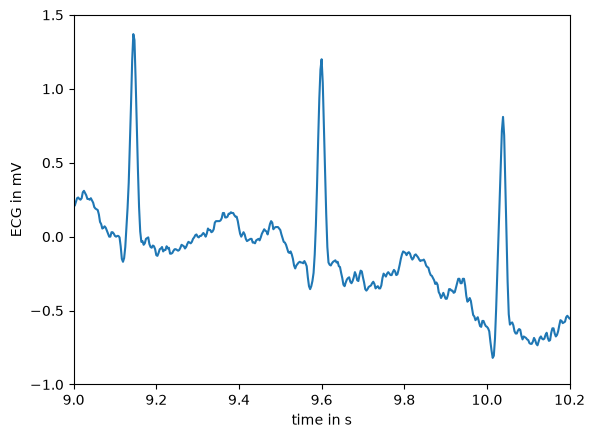
\includegraphics{443cf413-07a6-4db9-a47c-94fa47486bf5.png}

The signal was recorded at \textbf{fs = 360 Hz}, so
\texttt{time\ =\ np.arange(ecg.size)\ /\ fs} converts sample indices to
seconds.

\hypertarget{audio-recording-playback}{%
\subsubsection{Audio Recording \&
Playback}\label{audio-recording-playback}}

\hypertarget{recording-audio}{%
\paragraph{Recording Audio}\label{recording-audio}}

\begin{Shaded}
\begin{Highlighting}[]
\ImportTok{import}\NormalTok{ sounddevice}
\ImportTok{from}\NormalTok{ scipy.io.wavfile }\ImportTok{import}\NormalTok{ write}
\NormalTok{fs}\OperatorTok{=} \DecValTok{44100}
\NormalTok{second }\OperatorTok{=} \BuiltInTok{int}\NormalTok{(}\BuiltInTok{input}\NormalTok{(}\StringTok{"enter time duration in second:"}\NormalTok{))}
\BuiltInTok{print}\NormalTok{(}\StringTok{"recording..."}\NormalTok{)}
\NormalTok{record\_voice}\OperatorTok{=}\NormalTok{ sounddevice.rec(}\BuiltInTok{int}\NormalTok{(second }\OperatorTok{*}\NormalTok{ fs), samplerate}\OperatorTok{=}\NormalTok{fs, channels}\OperatorTok{=}\DecValTok{1}\NormalTok{)}
\NormalTok{sounddevice.wait()}
\NormalTok{write(}\StringTok{"output.wav"}\NormalTok{, fs, record\_voice)}
\BuiltInTok{print}\NormalTok{(}\StringTok{"recording complete"}\NormalTok{)}
\end{Highlighting}
\end{Shaded}

Records audio from the microphone for a user-specified duration at 44100
Hz and saves it as \texttt{output.wav}.

\hypertarget{listing-audio-devices}{%
\paragraph{Listing Audio Devices}\label{listing-audio-devices}}

\begin{Shaded}
\begin{Highlighting}[]
\NormalTok{sounddevice.query\_devices()}
\end{Highlighting}
\end{Shaded}

Lists all available audio input/output devices on the system.

\hypertarget{playback}{%
\subsubsection{Playback}\label{playback}}

Two ways to play back the saved file:

\begin{enumerate}
\def\labelenumi{\arabic{enumi}.}
\tightlist
\item
  \textbf{\texttt{sounddevice} + \texttt{soundfile}} --- reads the WAV
  and plays it via the system audio device
\end{enumerate}

\begin{Shaded}
\begin{Highlighting}[]
\ImportTok{import}\NormalTok{ sounddevice}
\ImportTok{import}\NormalTok{ soundfile }\ImportTok{as}\NormalTok{ sf}

\NormalTok{data, fs }\OperatorTok{=}\NormalTok{ sf.read(}\StringTok{"output.wav"}\NormalTok{, dtype}\OperatorTok{=}\StringTok{"float32"}\NormalTok{)}
\NormalTok{sounddevice.play(data, fs)}
\NormalTok{sounddevice.wait()}
\end{Highlighting}
\end{Shaded}

\begin{enumerate}
\def\labelenumi{\arabic{enumi}.}
\setcounter{enumi}{1}
\tightlist
\item
  \textbf{\texttt{IPython.display.Audio}} --- embeds an interactive
  audio player directly in the notebook
\end{enumerate}

\begin{Shaded}
\begin{Highlighting}[]
\ImportTok{from}\NormalTok{ IPython.display }\ImportTok{import}\NormalTok{ Audio}
\NormalTok{Audio(}\StringTok{"output.wav"}\NormalTok{)}
\end{Highlighting}
\end{Shaded}

\hypertarget{visualizing-the-audio-waveform}{%
\paragraph{Visualizing the Audio
Waveform}\label{visualizing-the-audio-waveform}}

\begin{Shaded}
\begin{Highlighting}[]
\NormalTok{fs }\OperatorTok{=} \DecValTok{44100}
\NormalTok{time }\OperatorTok{=}\NormalTok{ np.arange(data.size) }\OperatorTok{/}\NormalTok{ fs}
\NormalTok{plt.plot(time, data)}
\NormalTok{plt.xlabel(}\StringTok{"time in s"}\NormalTok{)}
\NormalTok{plt.ylabel(}\StringTok{"amplitude"}\NormalTok{)}
\NormalTok{plt.xlim(}\FloatTok{0.5}\NormalTok{, }\FloatTok{0.6}\NormalTok{)}
\NormalTok{plt.ylim(}\OperatorTok{{-}}\FloatTok{1.5}\NormalTok{, }\FloatTok{1.5}\NormalTok{)}
\NormalTok{plt.show()}
\end{Highlighting}
\end{Shaded}

Plots the amplitude of the audio signal over time, zoomed into a 100ms
window (0.5--0.6s).

\hypertarget{complex-numbers-reviewintro}{%
\subsubsection{Complex Numbers
(Review/Intro)}\label{complex-numbers-reviewintro}}

\hypertarget{complex-square-root}{%
\paragraph{Complex Square Root}\label{complex-square-root}}

\begin{Shaded}
\begin{Highlighting}[]
\NormalTok{cmath.sqrt(}\OperatorTok{{-}}\DecValTok{1}\NormalTok{)  }\CommentTok{\# → 1j}
\end{Highlighting}
\end{Shaded}

\hypertarget{defining-inspecting-a-complex-number}{%
\paragraph{Defining \& Inspecting a Complex
Number}\label{defining-inspecting-a-complex-number}}

\begin{Shaded}
\begin{Highlighting}[]
\NormalTok{z }\OperatorTok{=} \DecValTok{2} \OperatorTok{+} \OtherTok{3j}
\NormalTok{np.real(z)   }\CommentTok{\# 2.0}
\NormalTok{np.imag(z)   }\CommentTok{\# 3.0}
\NormalTok{np.}\BuiltInTok{abs}\NormalTok{(z)    }\CommentTok{\# magnitude}
\NormalTok{np.angle(z)  }\CommentTok{\# phase angle in radians}
\end{Highlighting}
\end{Shaded}

\hypertarget{visualizations}{%
\paragraph{Visualizations}\label{visualizations}}

\begin{itemize}
\tightlist
\item
  \textbf{Cartesian plot} --- plots \texttt{z} as a point on the
  real/imaginary plane with axes drawn
\end{itemize}

\begin{Shaded}
\begin{Highlighting}[]
\CommentTok{\# plot the complex number}
\NormalTok{plt.plot(np.real(z),np.imag(z), }\StringTok{\textquotesingle{}ks\textquotesingle{}}\NormalTok{)}

\CommentTok{\# make plot look nicer}
\NormalTok{plt.xlim([}\OperatorTok{{-}}\DecValTok{5}\NormalTok{,}\DecValTok{5}\NormalTok{])}
\NormalTok{plt.ylim([}\OperatorTok{{-}}\DecValTok{5}\NormalTok{,}\DecValTok{5}\NormalTok{])}
\NormalTok{plt.plot([}\OperatorTok{{-}}\DecValTok{5}\NormalTok{,}\DecValTok{5}\NormalTok{], [}\DecValTok{0}\NormalTok{,}\DecValTok{0}\NormalTok{],}\StringTok{\textquotesingle{}k\textquotesingle{}}\NormalTok{)}
\NormalTok{plt.plot([}\DecValTok{0}\NormalTok{,}\DecValTok{0}\NormalTok{], [}\OperatorTok{{-}}\DecValTok{5}\NormalTok{,}\DecValTok{5}\NormalTok{],}\StringTok{\textquotesingle{}k\textquotesingle{}}\NormalTok{)}
\NormalTok{plt.xlabel(}\StringTok{\textquotesingle{}real axis\textquotesingle{}}\NormalTok{)}
\NormalTok{plt.ylabel(}\StringTok{\textquotesingle{}imag axis\textquotesingle{}}\NormalTok{)}
\NormalTok{plt.show()}
\end{Highlighting}
\end{Shaded}

\begin{itemize}
\tightlist
\item
  \textbf{Polar plot} --- uses \texttt{plt.polar()} to draw a vector
  from the origin with its magnitude and angle
\end{itemize}

\begin{Shaded}
\begin{Highlighting}[]
\NormalTok{mag }\OperatorTok{=}\NormalTok{ np.}\BuiltInTok{abs}\NormalTok{(z)}
\NormalTok{ang }\OperatorTok{=}\NormalTok{ np.angle(z)}

\NormalTok{plt.polar([}\DecValTok{0}\NormalTok{, ang], [}\DecValTok{0}\NormalTok{, mag], }\StringTok{\textquotesingle{}r\textquotesingle{}}\NormalTok{)}
\NormalTok{plt.show()}
\end{Highlighting}
\end{Shaded}

\hypertarget{polynomial-roots}{%
\paragraph{Polynomial Roots}\label{polynomial-roots}}

\begin{Shaded}
\begin{Highlighting}[]
\NormalTok{p }\OperatorTok{=}\NormalTok{ [}\DecValTok{1}\NormalTok{, }\DecValTok{0}\NormalTok{, }\DecValTok{0}\NormalTok{, }\DecValTok{1}\NormalTok{]}
\NormalTok{np.roots(p)}
\end{Highlighting}
\end{Shaded}

Finds solutions to \(x^3 + 1 = 0\).
